\section{Overview of Supervised Learning}

\subsection{Introduction}
In learning problems, there is a set of variables that mighe be denoted as \textit{inputs}, which are measured or preset. These variables have some influence on one or more \textit{outputs}. The goal is to use the inputs to predict the values of the outputs. This type is called \textit{supervised learning}.

\subsection{Variable Types and Terminology}
In short, we will use $X$ as an input vector, and the $i$-th row of $X$ is $x_i^T$, the vector transpose of $x_i$. Our goal is to make a good prediction of the output $Y$, denoted by $\hat{Y}$. There are two different types of output: $\hat{Y}$ for real-value output and $\hat{G}$ categorical output.

\subsection{Two Simple Approaches to Prediction: Least Squares and Nearest Neighbors}
In this section, we provide two simple yet powerful preduction methods: the linear model fit by *least squares* and the method of $k$-nearest neighbors.

\subsubsection{Linear Models and Least Squares}
Given a vector of inputs $X^T = (X_1, X_2, \ldots, X_p)$, we predict the output $Y$ via the model
\begin{equation}
	\hat{Y} = \hat{\beta}_0 + \sum_{j=1}^{p}X_j\hat{\beta}_j = X^T\hat{\beta}
\end{equation}
The term $\hat{\beta}_0$ is usually called the *intercept*, also known as the ***bias*** in machine learning.

In the method of **least squares**, we pick the coefficients $\beta$ to monimize the residual sum of squares
\[
	\text{RSS}(\beta) = \sum_{i=1}^{N}(y_i - x_i^T\beta)^2
\]
\[
	X^T(y-X\beta) = 0
\]
which we can write in matrix notation as: $\text{RSS}(\beta) = (y - X\beta)^T(y-X\beta)$ where $X$ is an $N \times p$ matrix with each row an input vector, and $y$ is an $N$-vector of the outputs in the training set. Differentiating the equation above with respect to $\beta$, we obtain the **normal equations**:
If $X^TX$ is nonsingular, then the unique solution is given by
\[
	\hat{\beta} = (X^TX)^{-1}X^Ty
\]
\begin{wrapfigure}{l}{0.25\textwidth}
	\centering
	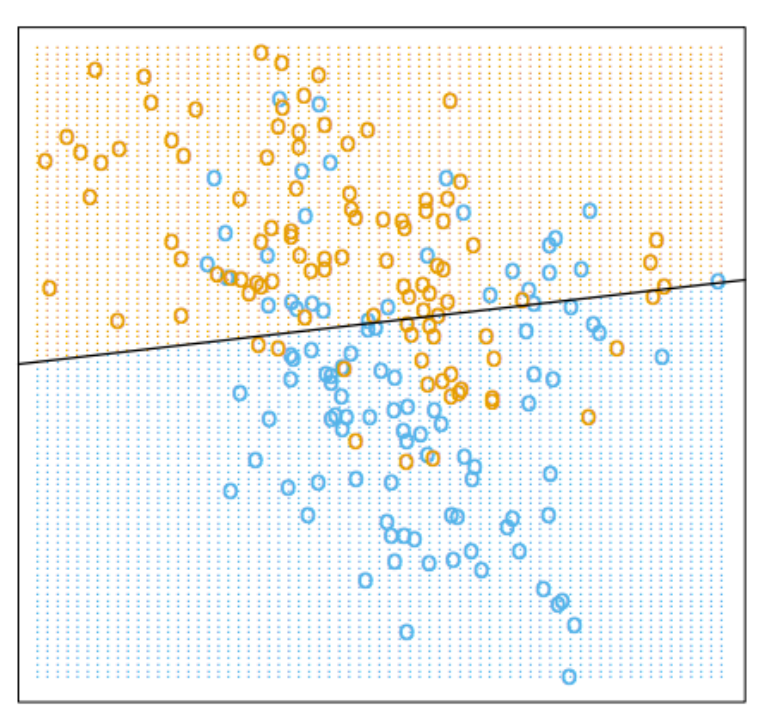
\includegraphics[width=0.25\textwidth]{2-1.png}
	\caption{}
\end{wrapfigure}
This example shows a two-dimension classification problems. The fitted line is formed using the *linear regression* method. The decision boundary is defined by $x^T\hat{\beta} = 0.5$.

Consider two possible scenarios:
\begin{itemize}
	\item The training data in each class were generated from bivariate Gaussian distributions with uncorrelated components and different means.
	\item The training data in each class came from a mixture of 10 low-variance Gaussian distributions, with individual means themselves distributed as Gaussian
\end{itemize}
For the second scenario, we'll see that a linear decision boundary is the best one can do, and that our estimate is almost optimal. However, for the first scenario, a linear decision boundary isn't likely to be optimal. The optimal decision boundary is nonlinear and disjoint, which will be much more difficult to obtain.

\subsubsection{Nearest-Neighbor Methods}
Specifically, the $k$-nearest neighbor fit for $\hat{Y}$ is defined as follows:
\[
	\hat{Y}(x) = \frac{1}{k}\sum_{x_i\inN_k(x)}y_i
\]
where $N_k(x)$ is the neighborhood of $x$ defined by the $k$ closest points $x_i$ in the training sample. So, in words, we find $k$ observations with $x_i$ closest to $x$ in input space, and average their responses. \\

\begin{wrapfigure}{l}{0.2\textwidth}
	\centering
	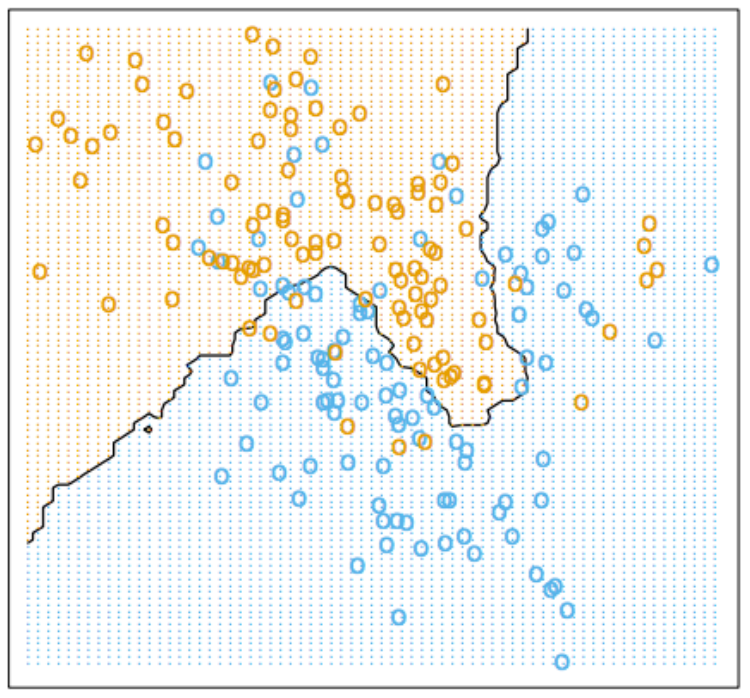
\includegraphics[width=0.2\textwidth]{2-2.png}
	\caption{}
\end{wrapfigure}

In this figure, it shows the same classification example fitted by 15-nearest-neighbor. We see that far fewer training observations are misclassified than that done by the *least squares* method. This doesn't show that the $k$-nearest neighbor classification is better than the *least squares*. Because when $k = 1$, it will create a high variance problem in the fit as shown in the next figure.


It appears that $k-$nearest neighbor fits have a single parameter, the number of neighbors $k$, compared to the $p$ parameters in least-squares fits. We'll see that the *effective* number of parameters of $k$-nearest neighbors is $N/k$ and is generally bigger than $p$.

It is clear that we cannot use sum-of-squared errors on the training set as a criterion for picking $k$, since we could always pick $k=1$ that results in the smallest value of errors. It seems that the $k$-nearest-neighbor method would be more appropriate for the mixture Scenario 2 described above, while for Gaussian data the decision boundaries of $k$-nearest neighbors would be unnecessarily noisy.

\begin{figure}
	\centering
	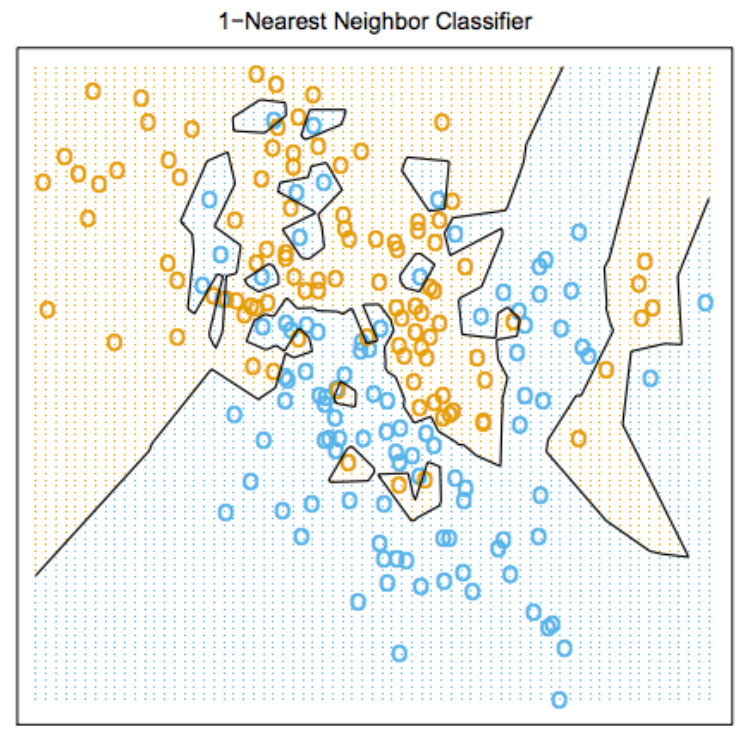
\includegraphics[width=0.5\textwidth]{2-3.png}
	\caption{}
\end{figure}

\subsubsection{From Least Squares to Nearest Neighbors}
In short, we develop an idea that the *least-square* method gives a smooth curve, which in other words is low variance and potentially high bias.

In contrast, the $k$-nearest-neighbor procedures do not seem to rely on stringent assumption about the underlying data, and can adapt to any situation. However, any particular subregion of the decision boundary depends on a hanful amount of input points and their particular positions, and is thus wiggly and unstable--high variance and low bias.

\begin{wrapfigure}{l}{0.3\textwidth}
	\centering
	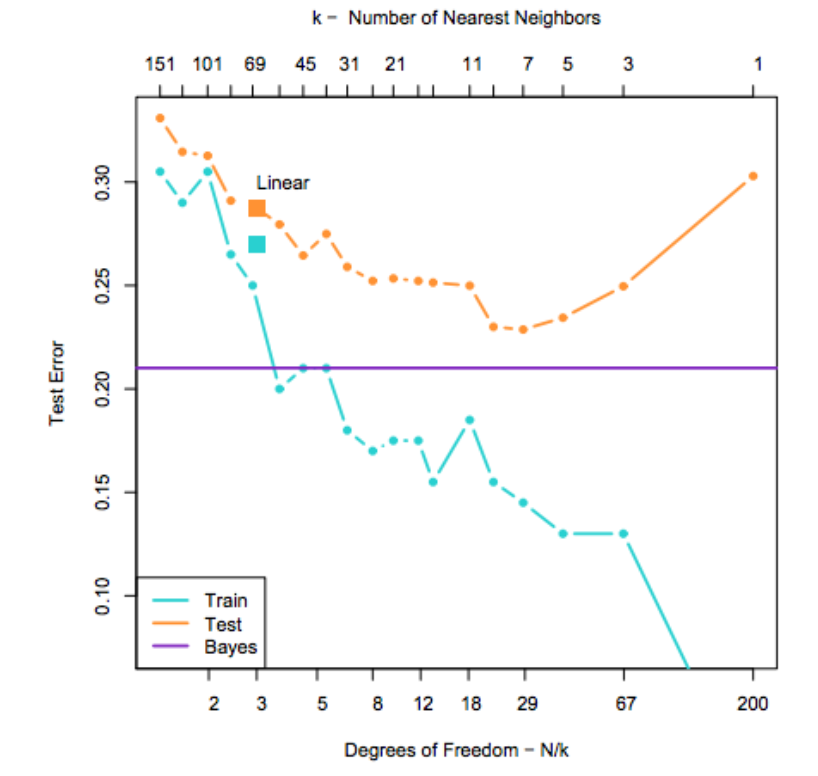
\includegraphics[width=0.3\textwidth]{2-4.png}
	\caption{}
\end{wrapfigure}

Each method has its own situations for which it works best. Provided that the data were ssimulated from a model somewhere between the two, but closer to Scenario 2. First, we generated 10 means $m_k$ from a bivariate Gaussian distribution $N((1,0)^T,I)$ and labeled this class as ***BLUE***. Similarly, 10 more were drawn from $N((0,1)^T,I)$ and labeled class ***ORANGE***. Then for each class we generated 100 observations as follows: for each observation, we picked an $m_k$ at random with probability $1/10$, and then generated a $N(m_k,I/5)$, thus leading to a mixture of Gaussian clusters for each class. This figure shows the result of classifying 10,000 new observations generated from the model. We compare the results for least squares and those for $k$-nearest neighbors for a range of values $k$.

The figure above shows the missclassification curves for the simulation example. A single training sample of size 200 was used, and a test sample of size 10,000. The *orange* curves are test and the *blue* are training error for $k$-nearest-neighbor classification. The purple line is the optimal Bayes error rate.

The following list describes some ways in which these simple procedures have been enhanced:
\begin{itemize}
	\item Kernel methods use weights that decrease smoothly to zero with distance from the target point, rather than the effective 0/1 weights used by $k$-nearest neighbors.
	\item In high-dimensional spaces the distance kernels are modified to emphasize some variable more than others
	\item Local regression fits linear models by locally weighted least squares, rather than fitting constants locally.
	\item Linear models fit to a basis expansion of the original inputs allow arbitrarily complex models.
	\item Projection pursuit and neural network models consist of sums of nonlinearly transformed linear models.
\end{itemize}

\subsection{Statistical Decision Theory}
We define the ***expected (squared) prediction error***:

\begin{align}
	\text{EPE}(f) &= \text{E}(Y - f(X))^2 \\
	&= \int [y - f(x)]^2 \Pr(dx,dy)
\end{align}
hello


\subsection{Local Methods in High Dimensions}

\subsection{Statistical Models, Supervised Learning and Function Approximation}

\subsubsection{A Statistical Model for the Jount Distribution $\Pr(X,Y)$}
\subsubsection{Supervised Learning}
\subsubsection{Function Approximation}

\subsection{Structured Regression Models}
\subsubsection{Difficulty of the Problem}
\subsection{Classes of Restricted Estimators}
\subsubsection{Roughness Penalty and Bayesian Methods}
\subsubsection{Kernel Methods and Local Regression}
\subsection{Model Selection and the Bias-Variance Tradeoff}


\subsection{Exercises}
